% !Mode:: "TeX:UTF-8"
\chapter{Backend: Part I}
\label{cpt:backend1}
\begin{mdframed}  
	\textbf{Goal of Study}
	\begin{enumerate}[labelindent=0em,leftmargin=1.5em]
		\item Learn how to formulate the backend problem into a filter or least square optimization problem.
		\item Learn how to use the sparse structure in bundle adjustment problem. 
		\item Solve a BA problem with g2o and Ceres.
	\end{enumerate}
\end{mdframed}

From this lecture, we turn to another important module: back-end optimization.
We see that the front-end visual odometry can give a short-term trajectory and map. Still, due to the inevitable accumulation of errors, this map is inaccurate for a long time. Therefore, based on visual odometry, we also hope to construct a larger-scale optimization problem to consider the optimal trajectory and map over a long time. However, considering the balance of accuracy and performance, there are many different approaches in practice.

\newpage
\includepdf{resources/other/ch10.pdf}

\newpage
\section{Introduction}
\subsection{State Estimation from Probabilistic Perspective}
As mentioned in the second lecture, the visual odometry only has a short memory, but we hope that the system can maintain the entire motion trajectory in an optimal state for a long time. We may use the latest knowledge to update an old state. At that time, it seems that future information tells you, ``where you should be now.'' Therefore, in the back-end optimization, we usually consider the problem of state estimation for a longer period of time (or all-time), and not only use the past information to update our current state but also use future information to update ourselves. Such a method might be called ``Batch.'' Otherwise, if the current state is only determined by the past, or even only by the previous moment, it might also be called ``Incremental.''

We already know that the SLAM process can be described by the motion and observation equations. Suppose in the time from $t=0$ to $t=N$, we have the poses from $\bm{x}_0$ to $\bm{x}_N$ and observation $\bm{y}_1, \cdots, \bm{y}_M$. According to the equations in chapter 2, we write them as: 
\begin{equation}
	\left\{ \begin{array}{l}
		{\bm{x}_k} = f\left( {{\bm{x}_{k - 1}},{\bm{u}_k}} \right) + \bm{w}_k \\
		{\bm{z}_{k,j}} = h\left( {{ \bm{y}_j},{ \bm{x}_k}}  \right)+ \bm{v}_{k,j}
	\end{array} \right. \quad k=1, \ldots, N, \  j=1, \ldots, M.
\end{equation}

Note that in the SLAM problem we have the following characteristics:
\begin{enumerate}
	\item In the observation equation, only when $\bm{x}_k$ sees $\bm{y}_j$, we will have a real observation equation. In fact, we can usually see only a small part of the landmarks in one location. Moreover, due to a large number of visual SLAM feature points, the number of observation equations in practice will be much larger than that of motion equations.
	\item We may not have a device to measure motion, so there may not be a motion equation. In this case, there are several ways to deal with it:
	\begin{itemize}
		\item Assume that there is really no motion equation.
		\item Assume that the camera does not move.
		\item Assume that the camera is moving at a constant speed.
	\end{itemize}
	These several methods are all feasible. In the absence of motion equations, the entire optimization problem consists of only observation equations. This is very similar to the SfM (Structure from Motion) problem, which is equivalent to restoring the motion and structure through a set of images. The difference with SfM is that the images in SLAM have a chronological order, while SfM allows the use of completely unrelated images.
\end{enumerate} 

We know that every measurement is affected by noise, so the poses $\bm{x}$ and landmarks $\bm{y}$ here are regarded as \textbf{random variables that obey a certain probability distribution} instead of a single number. Therefore, the question becomes: when I have some motion data $\bm{u}$ and observation data $\bm{z}$, how to determine the state $\bm{x}$ and landmarks $\bm{y}$'s distribution? Furthermore, if new data is obtained, how to update our estimation? In more common and reasonable cases, we assume that the state quantity and noise terms obey Gaussian distribution-which means that only their mean and covariance matrix need to be stored in the program. The mean can be regarded as an estimate of the state variable's optimal value, and the covariance matrix measures its uncertainty. Then, the question becomes: when there are some motion and observation data, how do we estimate the Gaussian distribution of the states?

We still put ourselves in the role of a robot. When there is only the equation of motion, it is equivalent to walking blindfolded in an unknown place. Although we know how far we have taken for each step, we will become more and more uncertain about where we are as time grows. This reflects that when the input data is affected by noise, the error is gradually accumulated, and our estimate of the position variance will become larger and larger. However, when we open our eyes, we will become more and more confident because we can continuously observe the external scene, making the uncertainty of position estimation smaller. If we use an ellipse to intuitively express the covariance matrix, then this process is a bit like walking in a mobile phone map software. Taking \autoref{fig:uncertainty}~ as an example, readers can imagine that when there is no observation data, the circle will become larger and larger with the movement; and if there are correct observations, the circle will shrink to a certain size and keep stable.

\begin{figure}[!ht]
	\centering
	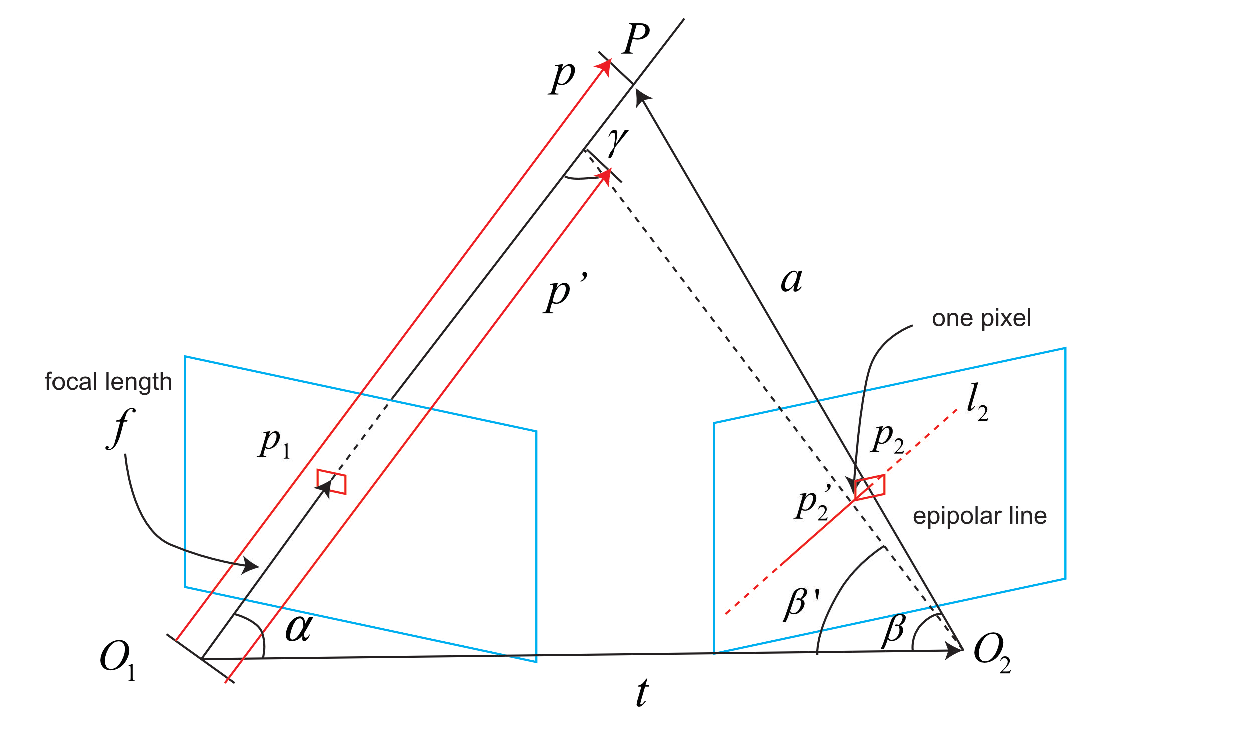
\includegraphics[width=0.66\textwidth]{backend1/uncertainty.pdf}
	\caption{An intuitive description of uncertainty. Left: When there is only the motion equation, the pose at the next moment adds noise to the previous moment, so the uncertainty is getting bigger and bigger. Right: When there are road signs, the uncertainty will be significantly reduced. Please note that this is only an intuitive diagram, not actual data.}
	\label{fig:uncertainty}
\end{figure}

The above statements explain the problem of state estimation in a metaphorical form. Below we will look at it in a quantitative way. In Lecture \ref{cpt:6}, we introduced the maximum likelihood estimation where we say that the problem of \textbf{batch state estimation} can be transformed into a \textbf{maximum likelihood estimation problem and solved by the least square method}. In this section, we will explore how to apply this conclusion to progressive problems and get some classic conclusions. At the same time, we will investigate the special structure of the least square method in visual SLAM.


